\documentclass[a4paper,11pt]{article}

\usepackage[T1]{fontenc}
\usepackage[french]{babel}
\usepackage{graphicx}
\usepackage{lmodern}
\usepackage[utf8]{inputenc}
\usepackage{parskip}
\usepackage{tikz}
\usetikzlibrary{arrows.meta, positioning}
\usepackage{float}
\usepackage[margin=2.5cm]{geometry}

\usepackage{listings}
\usepackage{xcolor}
\usepackage{textcomp}
\usepackage{upquote}

% Configuration du style
\lstset{
    language=Java,
    basicstyle=\ttfamily\small,
    backgroundcolor=\color{black!5},
    keywordstyle=\color{blue}\bfseries,
    stringstyle=\color{purple},
    commentstyle=\color{green!60!black}\itshape,
    numbers=none,
    rulecolor=\color{black!30},
    frame=single,
    breaklines=true,
    columns=fullflexible,
    keepspaces=true,
    showstringspaces=false,
    showspaces=false,
    upquote=true,
    extendedchars=true,
    morekeywords={String, System, Thread, Runnable, Exception, RuntimeException, Object},
    literate=
    {é}{{\'e}}1
    {è}{{\`e}}1
    {ê}{{\^e}}1
    {à}{{\`a}}1
    {â}{{\^a}}1
    {ç}{{\c{c}}}1
    {ù}{{\`u}}1
    {î}{{\^i}}1
    {ô}{{\^o}}1
    {'}{\textquotesingle}1
}

%Info document
\title{Rapport Projet - Programmation répartie}
\author{CERDA DE ALMEIDA VILACA Alexis\\ FOUSSE Emelyne \\ HERMANN Taïno \\ SAGET Logan \\ }
\date{Juin 2026}

\begin{document}

\maketitle
\tableofcontents
\newpage

% ===================================================
\section{Introduction}
% ===================================================

Lien du répertoire GIT : \texttt{https://github.com/HermannT88/projet\_rmi\_calcul\_parallele}

Ce projet a pour objectif de concevoir et de mettre en oeuvre une application de calcul parallèle distribué appliquée au rendu d'images par lancer de rayons. La synthèse d'images par cette méthode étant une tâche particulièrement gourmande en ressources CPU, l'approche retenue consiste à diviser l'image globale en une multitude de blocs indépendants. En exploitant l'architecture Java RMI, ces tâches sont distribuées à un ensemble de nœuds de calcul connectés à un service central. Cette parallélisation des données permet de réduire considérablement le temps global d'exécution en mutualisant la puissance de calcul de plusieurs machines connectées en réseau.

\newpage

% ===================================================
\section{Le raytracer local}
% ===================================================

\subsection{Mesures de temps d'exécution}

Pour réalisés des mesures sur le temps de calcul, nous avons fait une boucle qui exécute 10 fois le calcul de l'image avec à chaque itération \texttt{largeur = i * largeur de base} et \texttt{hauteur = i * hauteur de base}

\begin{lstlisting}
for (int i = 1; i<= 10; i++ ){
  int l = largeur*i, h = hauteur*i;
  
  Instant debut = Instant.now();
  System.out.println("Itération " + i + " Largeur = " + l + "Hauteur = "+ h);
  Image image = scene.compute(x0, y0, l, h);
  Instant fin = Instant.now();

  long duree = Duration.between(debut, fin).toMillis();
            
  System.out.println("Temps de calcul :"+duree+" ms");
}
\end{lstlisting}

Nous obtenons alors ces résultats :

\begin{table}[H]
\centering
\begin{tabular}{|c|c|c|c|}
\hline
\textbf{Itération} & \textbf{Largeur (px)} & \textbf{Hauteur (px)} & \textbf{Temps de calcul (ms)} \\
\hline
1 & 512 & 512 & 3182 \\
\hline
2 & 1024 & 1024 & 7372 \\
\hline
3 & 1536 & 1536 & 13642 \\
\hline
4 & 2048 & 2048 & 23977 \\
\hline
5 & 2560 & 2560 & 32773 \\
\hline
6 & 3072 & 3072 & 48813 \\
\hline
7 & 3584 & 3584 & 64370 \\
\hline
8 & 4096 & 4096 & 84049 \\
\hline
9 & 4608 & 4608 & 107256 \\
\hline
10 & 5120 & 5120 & 128906 \\
\hline
\end{tabular}
\caption{Évolution du temps de calcul en fonction des dimensions}
\end{table}

\vspace{0.5cm}
\begin{figure}[H]
  \noindent
  \begin{center}
  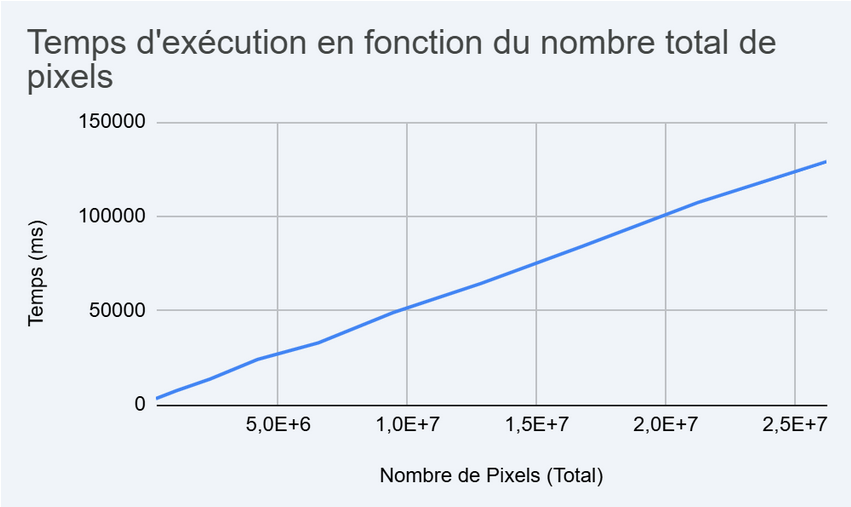
\includegraphics[width=\textwidth]{images/courbe.png}
  \end{center}
  \caption{\underline{Temps d'éxecution en fonction des pixels}}
\end{figure}
\vspace{0.5cm}

Nous constatons que le temps de calcul augmente proportionnelement au nombre de pixels de l'image.

\subsection{Reproduction de l'image}

L'objectif est de reproduire l'image ci-dessous :

\begin{figure}[H]
  \noindent
  \begin{center}
  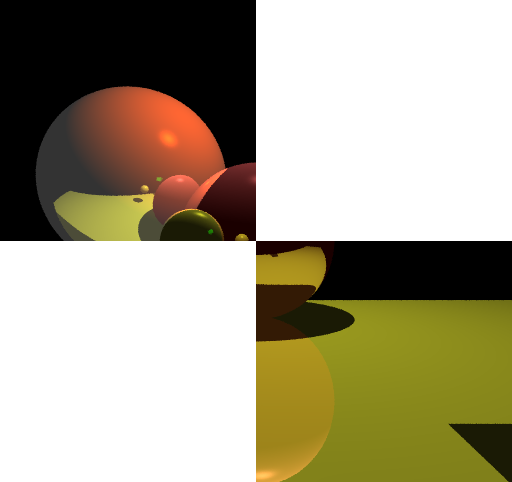
\includegraphics[width=7cm]{images/raytrace-resultat-2.png}
  \end{center}
  \caption{\underline{Image à reproduire}}
\end{figure}
\vspace{0.5cm}



Pour reproduire l'image, nous allons calculer individuellement les deux parties de l'image attendue.

La première partie, le programme va calculer l'image en partant des coordonnées 0 ; 0 soit le coin supérieur droit. Puis il va calculer l'image jusqu'a son centre, donc à la moitier de la hauteur et la moitier de la largeur. Ce qui nous donne la ligne suivante :

\begin{lstlisting}
  Image image1 = scene.compute(x0, y0, l/2, h/2);
\end{lstlisting}

Pour la seconde, nous allons recréé une image qui cette fois va commencer au millieu et encore avancé en largeur et en hauteur de la moitié. Nous avons alors cette ligne :

\begin{lstlisting}
  Image image2 = scene.compute(l/2, h/2, l/2, h/2);
\end{lstlisting}

Enfin nous affichons les deux images calculée précédemment sur la même fenêtre, avec la première au coordonnées 0 ; 0 et la seconde au centre de l'image :

\begin{lstlisting}
  disp.setImage(image1, x0, y0);
  disp.setImage(image2, l/2, h/2);
\end{lstlisting}

Pour le code complet, nous arrivons donc à ce résultat :

\begin{lstlisting}
int x0 = 0, y0 = 0;
int l = largeur, h = hauteur;

// Chronométrage du temps de calcul
Instant debut = Instant.now();
System.out.println("Calcul de l'image :\n - Coordonnées : "+x0+","+y0
+"\n - Taille "+ largeur + "x" + hauteur);
Image image1 = scene.compute(x0, y0, l/2, h/2);
Image image2 = scene.compute(l/2, h/2, l/2, h/2);
Instant fin = Instant.now();

long duree = Duration.between(debut, fin).toMillis();

System.out.println("Image calculée en :"+duree+" ms");

// Affichage de l'image calculée
disp.setImage(image1, x0, y0);
disp.setImage(image2, l/2, h/2);
\end{lstlisting}

\newpage

% ===================================================
\section{Architecture de l'application répartie}
% ===================================================

\subsection{Schéma de l'architecture}

Pour notre première idée d'architecture, l'application avait un client qui envoyait le fichier txt correspondant à l'image à calculer au service central. Ce service se serait ensuite chargé du découpage en threads et de la répartition entre les nœuds de calcul. Une fois l'image calculée entièrement, le service central aurait renvoyé l'objet Image au Client.

\begin{figure}[H]
  \noindent
  \begin{center}
  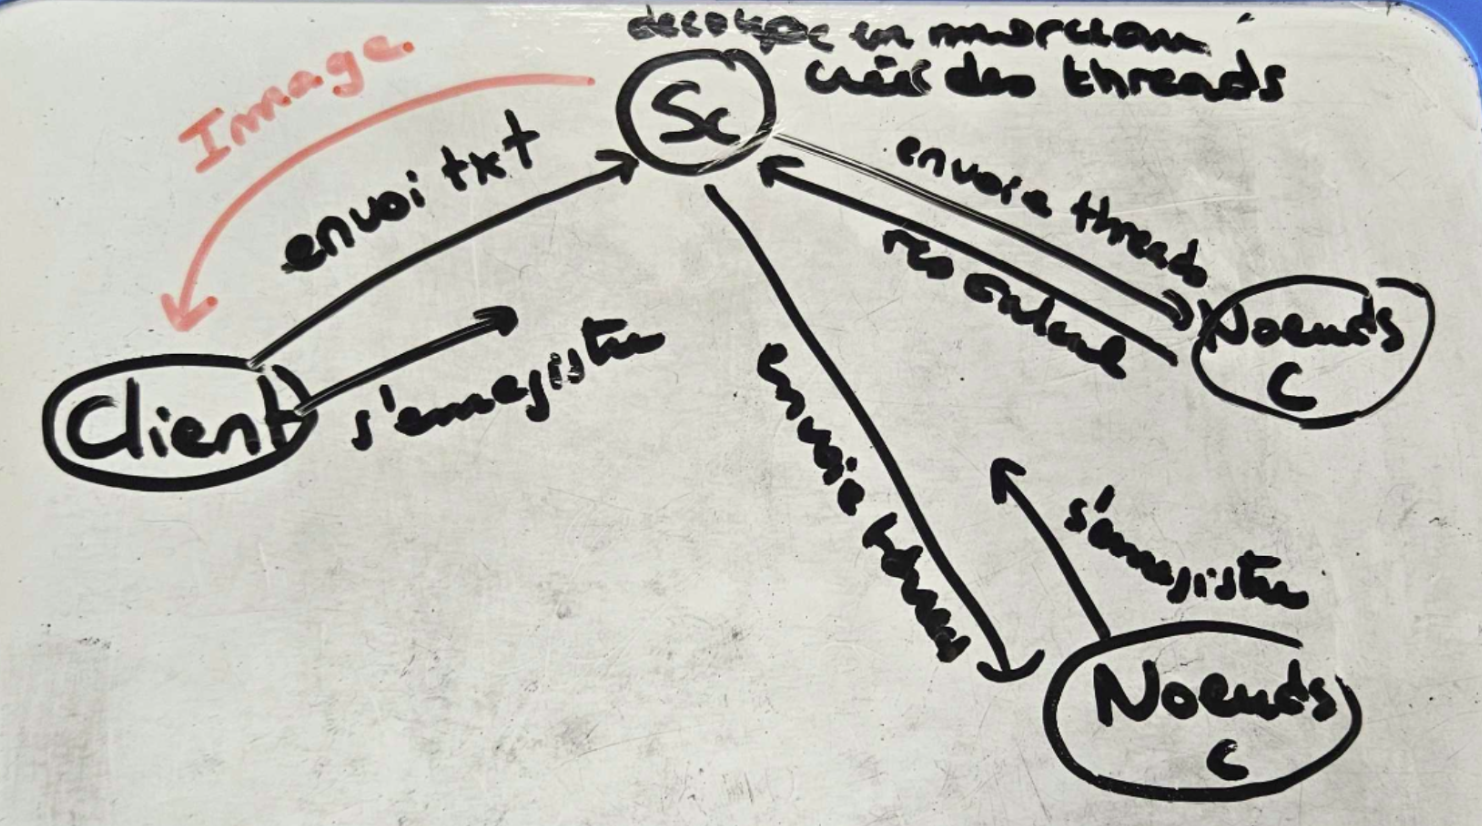
\includegraphics[width=12cm]{images/shema1.png}
  \end{center}
  \caption{\underline{Première version}}
\end{figure}
\vspace{0.5cm}

Pour la deuxième version, le fonctionnement était très similaire à la première version, avec cette fois toute la partie découpage des tâches et échanges avec les nœuds déléguée à un service Répartiteur.

\begin{figure}[H]
  \noindent
  \begin{center}
  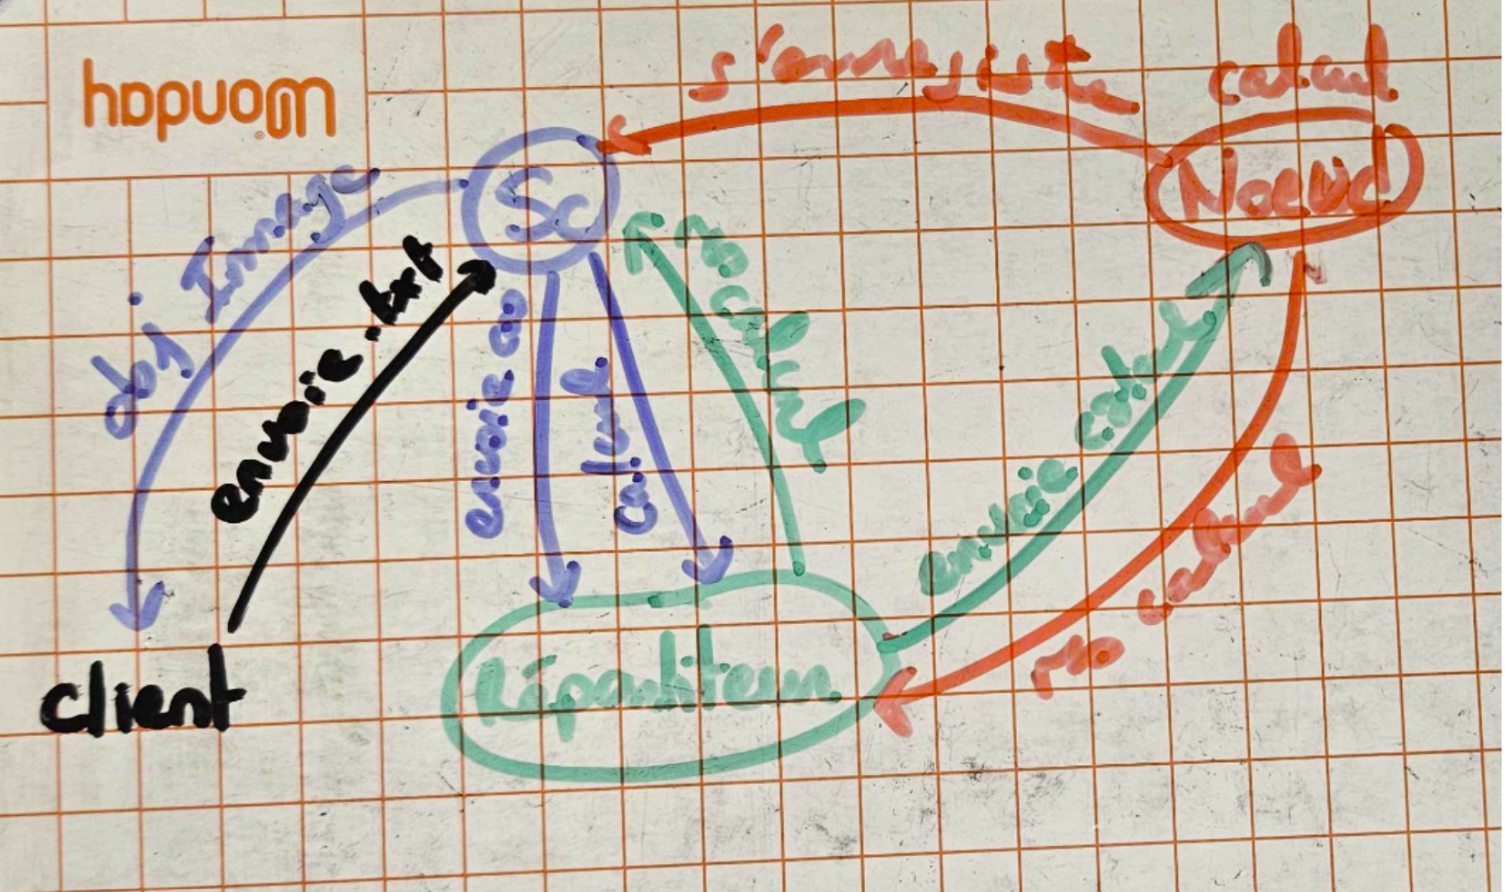
\includegraphics[width=12cm]{images/shema2.png}
  \end{center}
  \caption{\underline{Deuxième version}}
\end{figure}
\vspace{0.5cm}

Dans la version finale, toute la logique de découpage en threads a été redonnée au Client. Le service central ne sert plus qu'à fournir et gérer les nœuds, c'est-à-dire maintenir une liste de nœuds, en ajouter, en supprimer et envoyer un nœud lorsqu'un Client le demande.

\begin{figure}[H]
  \noindent
  \begin{center}
  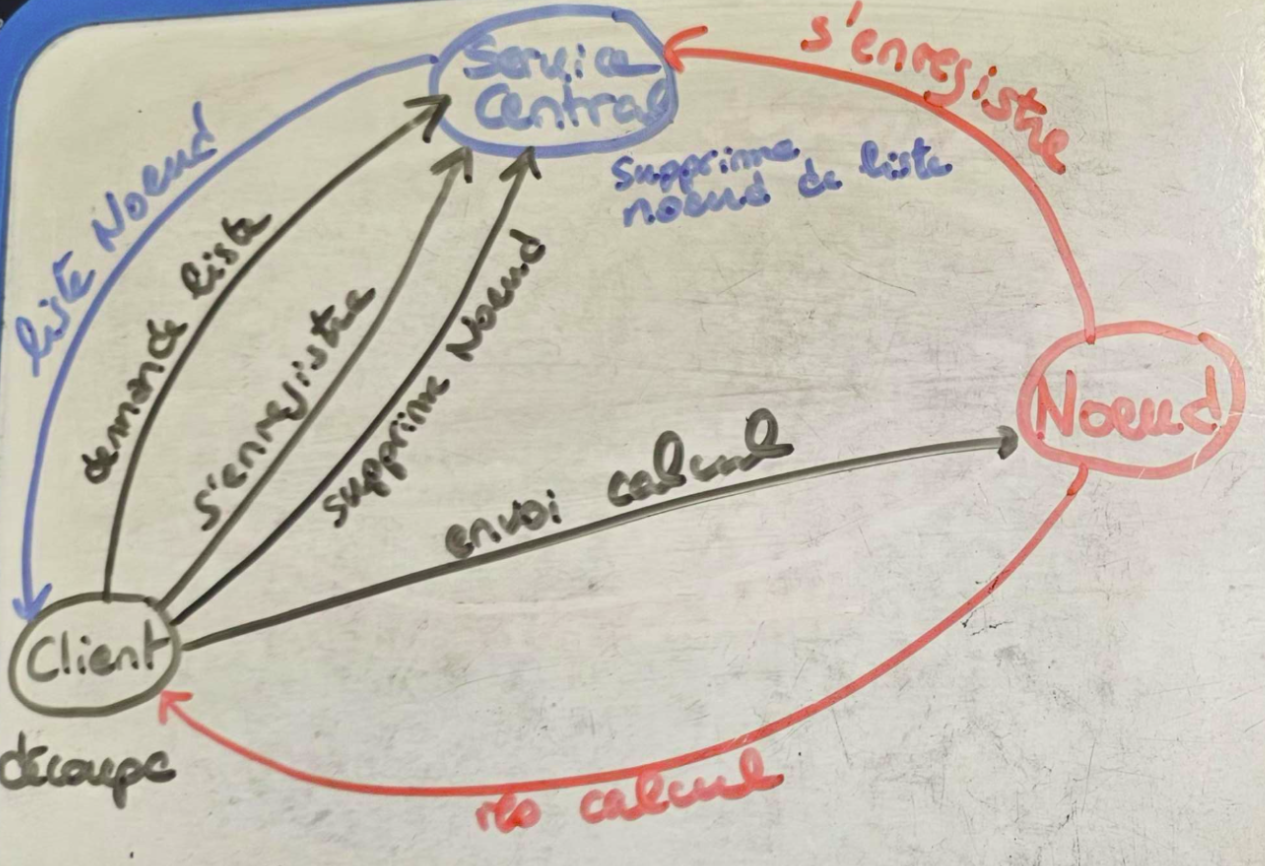
\includegraphics[width=12cm]{images/shema3.png}
  \end{center}
  \caption{\underline{Version finale}}
\end{figure}
\vspace{0.5cm}

* Contrairement à ce qui est indiqué sur le schéma, le service central renvoie un unique nœud au client et non la liste entière.

\subsection{Processus fixes et processus mobiles}

Dans notre architecture, nous pouvons distinguer deux types de processus en fonction de leur rôle et de leur cycle de vie sur le réseau :

Le processus fixe :
Le processus fixe est le Service Central. Il doit être lancé en premier et reste actif de manière permanente. Il écoute sur un port RMI défini (le port 1099 par défaut) et attend que d'autres processus s'y connectent pour tenir à jour son annuaire de nœuds de calcul.

Les processus mobiles :
Les processus mobiles apparaissent et disparaissent dynamiquement au cours du temps :
\begin{itemize}
    \item Les nœuds de calcul : Ils démarrent, s'enregistrent auprès du service central, et exposent leurs méthodes de calcul sur des ports dynamiques. Ils peuvent se déconnecter ou tomber en panne à tout moment.
    \item Le client : Il se connecte de manière éphémère lorsqu'il a une image à calculer. Il interroge le service pour obtenir les nœuds, effectue sa distribution de tâches en parallèle, puis se termine une fois l'image finale assemblée.
\end{itemize}

\subsection{Données échangées entre les processus}

Il est important de noter que le service central ne fait pas transiter les calculs d'images. Le client dialogue directement avec les nœuds. Voici les véritables échanges de données s'opérant dans le système :

\begin{itemize}
    \item Entre les nœuds et le Service Central : Les nœuds s'enregistrent en envoyant au service leur propre référence RMI (un stub) de type \texttt{ComputeNode}.
    \item Entre le Client et le Service Central : Le client demande à récupérer des nœuds de calcul. Le service lui retourne en réponse la référence distante d'un nœud disponible en appliquant une politique de round-robin.
    \item Entre le Client et les nœuds de calcul : C'est ici que se fait la transmission du travail lourd. Le client envoie directement aux nœuds le nom du fichier de description (ex: \texttt{simple.txt}), les coordonnées de départ du bloc à traiter ($x, y$), ses dimensions ($w, h$), ainsi que la taille totale de l'image.
    \item Entre les nœuds de calcul et le Client : Une fois le calcul d'un bloc terminé, le nœud retourne directement au client un objet sérialisable de type \texttt{Image} contenant les pixels calculés. Le client se charge ensuite de les assembler pour former le résultat final.
\end{itemize}

\newpage

% ===================================================
\section{Fonctionnement des composants}
% ===================================================

\subsection{Le service central}

Le service central agit comme un annuaire dynamique pour les ressources de calcul. Il implémente l'interface \texttt{ServiceInterface} et possède les rôles suivants :
\begin{itemize}
    \item \textbf{Registre des nœuds} : Il maintient une liste interne des nœuds de calcul actuellement connectés.
    \item \textbf{Gestion des connexions/déconnexions} : Il expose des méthodes \texttt{enregistrerNoeud} et \texttt{supprimerNoeud} pour mettre à jour cette liste.
    \item \textbf{Répartition de charge (Round-Robin)} : La méthode \texttt{obtenirNoeud()} distribue les nœuds disponibles de manière cyclique. Cela garantit qu'un client ne monopolise pas un seul nœud si plusieurs sont disponibles.
\end{itemize}
L'index du noeud distribuer est gérée de manière à boucler sur la liste des noeuds et à prendre en compte les nouveaux noeuds et les noeuds mort.

\subsection{Les nœuds de calcul}

Les nœuds de calcul sont les travailleurs de l'architecture. Chaque nœud est un programme autonome qui :
\begin{itemize}
    \item Instancie un objet implémentant l'interface \texttt{ComputeNode}.
    \item S'enregistre auprès du service central via RMI au démarrage.
    \item Expose une méthode distante \texttt{calculerBloc(...)} qui prend en paramètre le fichier de la scène, la position ($x, y$) du bloc à calculer, et ses dimensions ($w, h$).
    \item Instancie un moteur de \textit{raytracing} en mémoire, calcule les pixels correspondants à son bloc, et renvoie un objet \texttt{Image} (sérialisable) contenant le résultat.
\end{itemize}

Il y a aussi une classe LancerMultiNoeuds qui permet de créer puis lancer N noeuds dans des threads.

\subsection{Le client / dispatcher}

Le client est le programme qui souhaite rendre une image. Il joue un rôle actif de \textit{dispatcher} :
\begin{enumerate}
    \item Il se connecte au service central pour connaître les nœuds disponibles.
    \item Il divise l'image complète en plusieurs sous-parties indépendantes appelées "blocs" ou "tâches" (par exemple, un quadrillage 10x10).
    \item Il place toutes ces tâches dans une file de travail (une liste partagée).
    \item Il lance un thread "worker" local pour chaque nœud disponible.
    \item Un thread secondaire nommé "watcher" surveille périodiquement le service central pour détecter l'apparition de nouveaux nœuds et lancer des threads supplémentaires si nécessaire.
    \item Si un worker vient à mourir ou à se déconnecter, il tue son thread et renvoie le bloc en cours dans la file de travail.
\end{enumerate}

\newpage

% ===================================================
\section{Mise en œuvre du parallélisme}
% ===================================================

\subsection{Distribution des tâches en threads}

Pour exploiter les nœuds distants, le client génère un parallélisme local via des \texttt{Thread} Java. 
La liste des tâches (\texttt{fileTravail}) est gérée de manière synchronisée. Chaque thread local effectue la boucle suivante :
\begin{itemize}
    \item Il demande un nœud de calcul au service.
    \item Tant qu'il reste des blocs, il extrait un bloc via une méthode \texttt{prendreProchainBloc()}.
    \item Il effectue l'appel RMI synchrone \texttt{calculerBloc} sur son nœud attribué.
\end{itemize}

L'architecture gère également la tolérance aux pannes : si l'appel RMI échoue (par exemple si un nœud se déconnecte subitement), l'exception \texttt{RemoteException} est interceptée. Le client informe alors le service central de supprimer ce nœud, et le bloc inachevé est replacé dans la file via \texttt{remettreBloc(tache)}.

\subsection{Synchronisation et assemblage des résultats}

L'assemblage des sous-images (\texttt{Image} reçues des nœuds) dans l'image finale est géré par la méthode \texttt{recevoirResultat}. Cette méthode copie les pixels du bloc reçu vers l'image complète. 

Chaque noeuds appel cette méthode à chaque fois qu'ils terminent un bloc et donc l'ajout à l'image finale et actualise l'image en direct.

Pour éviter les problèmes d'accès concurrents lors de la modification de l'image globale et du compteur de blocs restants, le client utilise le mot-clé \texttt{synchronized}. De plus, le compteur \texttt{blocsRestants} est décrémenté à chaque résultat reçu. Lorsqu'il atteint 0, la méthode déclenche un \texttt{notifyAll()} pour réveiller le thread principal qui était en attente (bloqué par un \texttt{wait()}), signifiant ainsi la fin du calcul distribué. L'image est également actualisée en temps réel à l'écran via l'interface graphique \texttt{Disp}.

\newpage

% ===================================================
\section{Conclusion}
% ===================================================

La mise en place de RMI nous a permis de distribuer les lourds calculs de \textit{raytracing} sur un réseau d'ordinateurs. L'approche choisie se démarque par sa robustesse et sa flexibilité :
\begin{itemize}
    \item \textbf{Scalabilité horizontale} : L'ajout de nouveaux nœuds pendant le calcul est détecté automatiquement, ce qui accélère la résolution de l'image en temps réel.
    \item \textbf{Tolérance aux pannes} : Un ordinateur défaillant n'interrompt pas le rendu. Le bloc perdu est simplement réaffecté à un autre nœud.
\end{itemize}
En divisant judicieusement le travail en petites tâches et en évitant les verrous bloquants prolongés, le temps de calcul est drastiquement réduit, offrant des performances bien supérieures à un calcul purement local.

\end{document}